\section{Uma variável aleatória contínua}

Considere uma \va\ $X$ contínua. Defina a \va\ $Y = H(X)$,
sendo $H$ uma função \textit{contínua},
de modo que $Y$ também é contínua.
Vamos considerar dois casos a seguir.

Em todos os casos, a função densidade de $X$ é $f_X(x)$,
a função de distribuição acumulada é $F_X(x)$ e $A_X$ é o conjunto
de valores para os quais $f_X(x) > 0$, ou seja:
\begin{align*}
    A_X &= \{x \in \R: f_X(x) > 0\}.
\end{align*}

\subsection{Método da função de distribuição acumulada}

Pela \cref{def:ch02-fda}, a função de distribuição acumulada de $Y$ é
\begin{align*}
    F_Y(y) &= \Prob(Y \le y) \\
    &\overset{Y = H(X)}{=} \Prob(H(X) \le y)
\end{align*}
Se $H$ é bijetora e crescente, podemos escrever
\begin{align}
    F_Y(y) &= \Prob(H(X) \le y) \notag \\
    &= \Prob(X \le H^{-1}(y)) \notag \\
    &= F_X(H^{-1}(y)) \notag \\
    \therefore F_Y(y) &= F_X(H^{-1}(y))
    \label{eq:ch04-metodo-fda-simpl}
\end{align}

Considere uma função $H$ mais geral (contínua, mas não
necessariamente bijetora ou crescente), como ilustrada na 
\cref{fig:ch04-h-geral}.

\begin{figure}[!ht]
    \centering
    \begin{tikzpicture}
    \end{tikzpicture}
\end{figure}

\begin{figure}[!ht]
    \centering
    \begin{tikzpicture}

        \draw[->,>=stealth, thick] (-6, 2) -- (6, 2);
        \node[anchor=west] at (6, 2) {$X$};
        
        \draw[->,>=stealth, thick] (-6, -2) -- (6, -2);
        \node[anchor=west] at (6, -2) {$Y$};

        \coordinate (X1) at (-3,2);
        \coordinate (X2) at (0,2);
        \coordinate (X3) at (2,2);
        
        \coordinate (Y1) at (-4,-2);
        \coordinate (Y2) at (3,-2);
        \coordinate (Y3) at (-1,-2);
        
        \coordinate (y) at (1,-2);

        \draw[ultra thick, red] ($(X1)-(1,0)$) -- ($(X3)+(1,0)$);
        \draw[fill,red] ($(X1)-(1,0)$) circle (.5ex);
        \draw[fill,red] ($(X3)+(1,0)$) circle (.5ex);
        \node[anchor=south, red] at (-.5,2) {$A_X$};
        
        \draw[ultra thick, red] ($(Y1)-(1,0)$) -- ($(Y2)+(1,0)$);
        \draw[fill,red] ($(Y1)-(1,0)$) circle (.5ex);
        \draw[fill,red] ($(Y2)+(1,0)$) circle (.5ex);
        \node[anchor=south, red] at (-.5,-2) {$A_Y$};

        \node[anchor=north, yshift=-1ex] at (X1) {$x_1$};
        \node[anchor=north, yshift=-1ex] at (X2) {$x_2$};
        \node[anchor=north, yshift=-1ex] at (X3) {$x_3$};

        \node[anchor=north, yshift=-1ex] at (Y1) {$y_1 = H(x_1)$};
        \node[anchor=north, yshift=-1ex] at (Y2) {$y_2 = H(x_2)$};
        \node[anchor=north, yshift=-1ex] at (Y3) {$y_3 = H(x_3)$};

        \foreach \i in {1,2,3} {
            \draw[thick] ($(X\i)+(0,.5ex)$) -- ($(X\i)-(0,.5ex)$);
            \draw[thick] ($(Y\i)+(0,.5ex)$) -- ($(Y\i)-(0,.5ex)$);
        }

        \draw[line width=.5ex,
            blue,
            dash pattern=on 1ex off 2ex]
            (-6, -2) -- (y);
        \draw[fill,blue] (y) circle (.5ex);
        \node[anchor=north, yshift=-1ex,blue] at (y) {$y$};

        \foreach \i / \out in {1/-150,2/-30,3/-150} {
            \draw[-latex] ($(X\i)$) 
                to[out=\out, in=90]
                ($(Y\i)+(0,1ex)$);
        }
    \end{tikzpicture}
    \caption{$x \mapsto H(x)$}
    \label{fig:ch04-h-geral}
\end{figure}

Temos
\begin{align}
    F_Y(y) &= \Prob(Y \le y) \notag \\
    &\overset{Y = H(X)}{=} \Prob(H(X) \le y) \notag \\
    &= \Prob(X \in B(y)) \label{eq:ch04-metodo-fda}
\end{align}
em que
\begin{align}
    B(y) &= \{
        x \in A_X: H(x) \le y
    \}. \label{eq:ch04-metodo-fda-dom}
\end{align}
Continuando, temos:
\begin{align*}
    F_Y(y) &= \int_{B(y)} f_X(x) \wrt x
\end{align*}

A função densidade de $Y$ é (\cref{eq:ch02-fda-fdp})
\begin{align*}
    f_Y(y) &= \diff{}{y} F_Y(y)
\end{align*}
para $y \in A_Y$. O conjunto $A_Y$ dos valores para os quais $f_Y(y) > 0$ é determinado pela transformação $H$.

Esse método é chamado de \textbf{método da função distribuição acumulada}.

\subsection{Método do jacobiano}

Considere, agora, que $H$ é contínua, monótona (crescente ou decrescente) e derivável. Deste modo, $H$ é inversível,
e sua inversa é $H^{-1}(x)$.

Pelo \textbf{método do jacobiano}:
\begin{align}
    f_Y(y) &= f_X(H^{-1}(y)) \cdot \left|\diff{H^{-1}(y)}{y}\right|
    \label{eq:ch04-metodo-jac}
\end{align}

\begin{example}
    Note que $H$ não é monótona ($A_X = \R$). No entanto,
    ela possui partes monótonas, e esses trechos estão definidos
    em subconjuntos disjuntos de $A_X$.
    
    \begin{center}
        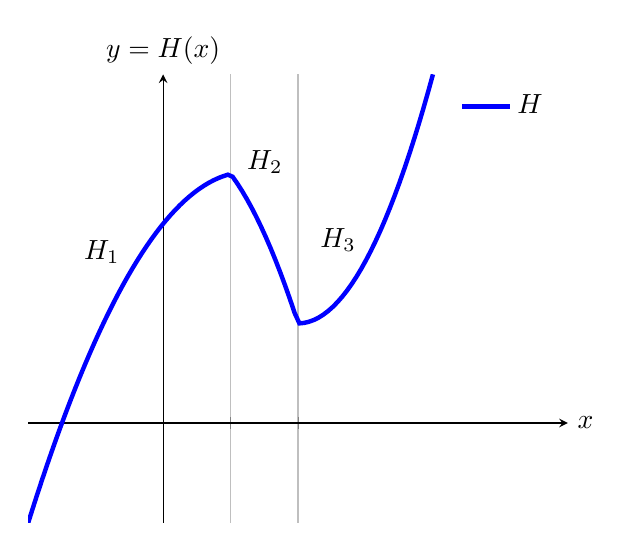
\begin{tikzpicture}[
            declare function={
                h1(\x) = -(2/3)*\x^2+(5/3)*\x+4;
                h2(\x) = -(6/5)*\x^2+(3/5)*\x+(28/5);
                h3(\x) = (5/4)*\x^2-5*\x+7;
                h(\x) = 
                    (\x < 1) * h1(\x) +
                    and(\x >= 1, \x < 2) * h2(\x) +
                    (\x > 2) * h3(\x);
            }
        ]
            \begin{axis}[
                unbounded coords=jump,
                grid=major,
                axis x line=middle,
                axis y line=middle,
                xmin=-2, xmax=6,
                ymin=-2, ymax=7,
                xtick={1,2},
                ytick=\empty,
                xticklabels=\empty,
                xlabel={$x$},
                ylabel={$y = H(x)$},
                x label style={anchor=west},
                y label style={anchor=south},
                legend style={fill=none,draw=none},
            ]

            \addplot[ultra thick, blue, samples=100, domain=-3:4] 
                {h(x)};
            \addlegendentry{$H$};

            \node[anchor=south east] at (-0.5,{h(-0.5)}) {$H_1$};
            \node[anchor=south west] at (1.1,{h(1.1)}) {$H_2$};
            \node[anchor=south east] at (3,{h(3)}) {$H_3$};
            \end{axis}
        \end{tikzpicture}
    \end{center}
\end{example}

Se o conjunto $A_X$ puder ser dividido em $k$ subconjuntos
disjuntos nos quais $H$ é monótona, temos:
\begin{align}
    f_Y(y) &= \sum_{j=1}^k
        f_X(H_j^{-1}(y)) \cdot \left|\diff{H_j^{-1}(y)}{y}\right|
    \label{eq:ch04-metodo-jac-partes}
\end{align}
em que $H_j$ indica cada parte monótona de $H$,
$j = 1, 2, \cdots, k$.

\begin{example}
    A \va\ $X$ representa o comprimento do raio de um círculo,
    com função densidade
    \begin{align*}
        f_X(x) &= \begin{cases}
            \frac{1}{R} &,\ \text{se } 0 < x < R \\
            0           &,\ \text{caso contrário.}
        \end{cases}
    \end{align*}
    A área do círculo de raio igual a $X$ é $Y = \pi X^2$.
    Deseja-se calcular a função densidade de $Y$.

    \bigskip
    Note que $A_X = (0, R)$. Além disso, $Y = H(X)$,
    com $H(X) = \pi X^2$, de modo que $Y \in (0, \pi ^2)$
    
    Como $H$ é monótona e derivável em $A_X$, podemos usar
    o \textbf{método do jacobiano}. Temos:
    \begin{align*}
        f_Y(y) &= f_X(H^{-1}(y)) 
            \cdot \left|\diff{H^{-1}(y)}{y}\right|
    \end{align*}
    em que
    \begin{align*}
        X &= H^{-1}(Y) \\
        &= \sqrt{\frac{Y}{\pi}}
    \end{align*}
    e
    \begin{align*}
        \diff{H^{-1}(y)}{y}
        &= \frac{1}{2\sqrt{\pi y}}
    \end{align*}
    em que $0 < y < \pi R^2$.

    Calculamos
    \begin{align*}
        f_Y(y) 
        &= f_X(H^{-1}(y)) 
            \cdot \left|\diff{H^{-1}(y)}{y}\right| \\
        &= \frac{1}{R} \cdot \left|\frac{1}{2\sqrt{\pi y}}\right| \\
        &= \frac{1}{2R\sqrt{\pi y}}
    \end{align*}
    com $0 < y < \pi R^2$.

    \begin{center}
        \begin{tikzpicture}[
            declare function={
                f(\x) = 1/(2*(pi*\x)^0.5);
            }
        ]
            \begin{axis}[
                unbounded coords=jump,
                grid=none,
                axis x line=middle,
                axis y line=middle,
                xmin=-0.5, xmax=4,
                ymin=0, ymax=1,
                xtick={pi},
                ytick={1/(2*pi)},
                xticklabels={$\pi R^2$},
                yticklabels={$\sfrac{1}{2\pi R^2}$},
                xlabel={$y$},
                ylabel={$f_Y(y)$},
                x label style={anchor=west},
                y label style={anchor=south},
                legend style={fill=none,draw=none},
            ]

            \addplot[ultra thick, blue, samples=100, domain=0.1:pi] 
                {f(x)};
            \addplot[ultra thick, blue, samples=2, domain=-0.5:0] 
                {0};
            \addplot[ultra thick, blue, samples=2, domain=pi:4] 
                {0};

            \addplot[ultra thick, blue, only marks] 
                coordinates {(0, 0) (pi, 0)};
            \addplot[ultra thick, blue, only marks, fill=white] 
                coordinates {(pi, {f(pi)})};

            \end{axis}
        \end{tikzpicture}
    \end{center}

    \bigskip
    Também é possível utilizar o \textbf{método da função de distribuição acumulada}. Temos (pela \cref{eq:ch04-metodo-fda-simpl}):
    \begin{align*}
        F_Y(y) &= F_X(H^{-1}(y))
    \end{align*}
    em que 
    \begin{align*}
        x = H^{-1}(y) &= \sqrt{\frac{y}{\pi}}
    \end{align*}
    e
    \begin{align*}
        F_X(x) &= \begin{cases}
            0 &,\ \text{se } x \le 0 \\
            \frac{x}{R} &,\ \text{se } 0 < x < R \\
            1 &,\ \text{se } x \ge R.
        \end{cases}
    \end{align*}

    Deste modo:
    \begin{align*}
        F_Y(y) &= F_X(H^{-1}(y)) \\
        &= \begin{cases}
            0 &,\ \text{se } H^{-1}(y) \le 0 \\
            \frac{H^{-1}(y)}{R} &,\ \text{se } 0 < H^{-1}(y) < R \\
            1 &,\ \text{se } H^{-1}(y) \ge R.
        \end{cases} \\
        &= \begin{cases}
            0 &,\ \text{se } \sqrt{\frac{y}{\pi}} \le 0 \\
            \frac{\sqrt{\frac{y}{\pi}}}{R} 
                &,\ \text{se } 0 < \sqrt{\frac{y}{\pi}} < R \\
            1 &,\ \text{se } \sqrt{\frac{y}{\pi}} \ge R.
        \end{cases} \\
        \therefore F_Y(y) &= \begin{cases}
            0 &,\ \text{se } y \le 0 \\
            \sqrt{\frac{y}{\pi R^2}}
                &,\ \text{se } 0 < y < \pi R^2 \\
            1 &,\ \text{se } y \ge \pi R^2.
        \end{cases}
    \end{align*}

    \begin{center}
        \begin{tikzpicture}[
                declare function={
                    F(\x) = sqrt(\x/pi);
                }
            ]
            \begin{axis}[
                unbounded coords=jump,
                grid=major,
                axis x line=middle,
                axis y line=middle,
                xmin=-0.5, xmax=4,
                ymin=0, ymax=1.1,
                xtick={pi},
                ytick={1},
                xticklabels={$\pi R^2$},
                xlabel={$y$},
                ylabel={$F_Y(y)$},
                x label style={anchor=south west},
                y label style={anchor=south},
                legend style={fill=none,draw=none},
            ]

            \addplot[ultra thick, blue, samples=100, domain=0:pi] 
                {F(x)};
            \addplot[ultra thick, blue, samples=2, domain=-.5:0] 
                {0};
            \addplot[ultra thick, blue, samples=2, domain=pi:4] 
                {1};

            \end{axis}
        \end{tikzpicture}
    \end{center}

    Derivando $F_Y(y)$, obtemos:
    \begin{align*}
        f_Y(y) = \diff{}{y} F_Y(y) &= \begin{cases}
            \diff{}{y} \sqrt{\frac{y}{\pi R^2}}
                &,\ \text{se } 0 < y < \pi R^2 \\
            0 &,\ \text{caso contrário.}
        \end{cases} \\
        \therefore f_Y(y) &= \begin{cases}
            \frac{1}{2R\sqrt{\pi y}}
                &,\ \text{se } 0 < y < \pi R^2 \\
            0 &,\ \text{caso contrário.}
        \end{cases}
    \end{align*}

    Como esperado, ambos os métodos conduziram ao mesmo resultado.
\end{example}

\begin{example}
    Temos
    \begin{align*}
        f_X(x) &= \begin{cases}
            \frac{1}{2} &,\ -1 < x < 1 \\
            0 &,\ \text{caso contrário.}
        \end{cases}
    \end{align*}

    Considere $Y = H(X) = X^2$; portanto, $Y \in (0, 1)$.

    Determinar a função densidade de $Y$.

    \bigskip
    Note que $H$ não é monótona; por isto, vamos usar
    o \textbf{método da função de distribuição acumulada}.

    \begin{obs}
        $H$ é monótona por partes, de modo que
        é possível utilizar o método do jacobiano
        nestas partes (a saber, $(-1, 0)$ e $[0, 1)$, por exemplo),
        de modo que é possível usar a
        \cref{eq:ch04-metodo-jac-partes} para encontrar
        a função densidade de $Y$.
    \end{obs}
    
    Como $Y \in (0, 1)$, sabemos que $f_Y(y) = 0$ se 
    $y \notin (0, 1)$. Tomamos, então, $y \in (0, 1)$ e calculamos:
    \begin{align*}
        F_Y(y) &= \Prob(Y \le y) \\
        &= \Prob(X^2 \le y) \\
        &= \Prob(-\sqrt{y} \le X \le \sqrt{y}) \\
        &= F_X(\sqrt{y}) - F_X(-\sqrt{y})
    \end{align*}

    \begin{obs}
        Note que o mesmo resultado seria obtido ao fazer
        \begin{align*}
            F_Y(y) &= \Prob(Y \le y) \\
            &= \Prob(X^2 \le y) \\
            &= \Prob(X \in B(y))
        \end{align*}
        em que
        \begin{align*}
            B(y) &= \{x \in (-1, 1) : x^2 \le y \} \\
            B(y) &= \{x \in (-1, 1) 
                : -\sqrt{y} \le x \le \sqrt{y} \} \\
        \end{align*}
        donde calculamos
        \begin{align*}
            F_Y(y) = \Prob(X \in B(y))
            &= \int_{B(y)} f_X(x) \wrt x
            = \int_{-\sqrt{y}}^{\sqrt{y}} f_X(x) \wrt x \\
            &= \left.F_X(x)\right|_{x=-\sqrt{y}}^{x=\sqrt{y}}
            = F_X(\sqrt{y}) - F_X(-\sqrt{y})
        \end{align*}
    \end{obs}

    Derivando $F_Y(y)$, obtemos:
    \begin{align*}
        f_Y(y) = \diff{}{y} F_Y(y)
        &= \diff{}{y} \left(F_X(\sqrt{y}) - F_X(-\sqrt{y})\right) \\
        &= f_X(\sqrt{y}) \cdot \frac{1}{2\sqrt{y}}
        - f_X(-\sqrt{y}) \cdot \left(-\frac{1}{2\sqrt{y}}\right) \\
        &= \frac{1}{2\sqrt{y}} \cdot
            \left\{f_X(\sqrt{y}) + f_X(-\sqrt{y})\right\} \\
        &= \frac{1}{2\sqrt{y}} \cdot
            \left\{\frac{1}{2} + \frac{1}{2}\right\} \\
        &= \frac{1}{2\sqrt{y}}
    \end{align*}
    para $0 < y < 1$.
\end{example}
